%!TEX root = ../paper.tex

\subsection{Clustering}
\label{sec:clustering}

After extracting all features and vectorising them for each blog post in our data set, we group them into clusters according to the similarity of their feature vectors.
Thus, the blog posts are grouped by their writing style into clusters.
One cluster represents one writing style, so that one cluster contains only blog posts with similar writing styles.


To this end, we use a \textit{k-means} algorithm, which is a method from vector quantization.
\textit{K-means} is one of the most popular and simplest clustering algorithms.
Using a \textit{k-means} algorithm the number of resulting clusters can be configured easily.


To run a \textit{k-means} algorithm, the value $k$ has to be set beforehand.
$K$ represents the number of clusters and thus the number of similar writing styles, which should be determined.
Depending on the value of $k$ the use case can differ.
Setting the value $k$ similar to the number of expected authors, the exact author should be found.
If $k$ is equal to the number of authors, one cluster, i.e. writing style group, would correspond to one author.
So one cluster would contain only blog posts of one author.
Choosing a value much lower than the actual number of authors for $k$, would allow us to find similar authors.
In this case, one cluster would contain blog posts from multiple authors having a similar writing style.



\subsection{Cluster Labelling}
\label{sec:cluster_labeling}

Labelling the resulting clusters helps the user to distinguish between them.
The labels indicate what kind of blog posts are in those clusters, so that the user gets an idea what to expect from blog posts in this cluster.


A lot of current research in the field of cluster labelling focuses on topic-dependent labels.
Because we want to cluster by writing style rather than topic, we were unable to use those techniques.
However, trying to find universally accepted writing styles leads to labels, such as ``informative'' or ``opinion piece'', which merely represent the text's intention, not the author's personal style~\cite{lee2001genres}.
Thus, these types of labels were also not applicable for our use case.


Therefore, we implemented our own cluster labelling methods, which consider the most important features of a cluster.
They will be explained using the following example:
The current feature is ``length of blog posts'' and we have three clusters with the following values for the feature:
\begin{center}
\begin{tabular}{c|c|c}
  Cluster 1 & Cluster 2 & Cluster 3 \\ \hline
  0.7 & 1 & 0.1 \\
 \end{tabular}
\end{center}


\paragraph{Method 1}
For each feature and cluster, the highest and lowest value is determined.
Those clusters are then given the appropriate labels.

In the example cluster 2 has the highest value and gets the label ``longest blog posts''.
The label ``shortest blog posts'' is assigned to cluster 3, because this cluster has the lowest value.

Using this method only the most significant labels are set.
But a cluster may not obtain any label when it does not have any extreme features.


\paragraph{Method 2}
First, the average vector of all blog posts is calculated.
In a second step, the distance for each feature and cluster to that average vector is determined.
If the distance is over or below a certain threshold, the cluster is labelled.

The example is shown in Figure~\ref{fig:cluster_labeling_2}.
Because cluster 3 is not over or below the threshold, thus the length of the blog post is not significant for the cluster, no label is assigned to that cluster.
Cluster 1 and 2 are both over the threshold and obtain the label ``long blog posts''.

This method assigns more labels to clusters than method 1, but can also lead to clusters without any labels if all of a cluster's feature have average values.

\begin{figure}[ht!]
	\centering
	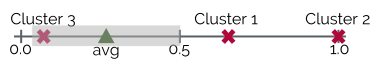
\includegraphics[width=0.6\textwidth]{images/cluster_labeling_2.pdf}
	\caption{Cluster labelling method 2: The distance of each cluster to the overall average blog posts is calculated. If the distance is over or below a certain threshold (shaded in grey), the cluster obtains a label. In this example a label is assigned to cluster 1 and 2.}
	\label{fig:cluster_labeling_2}
\end{figure}


\paragraph{Method 3}
Similarly to method 2, we look at each feature and discern the average for that feature.
We then calculate the difference between this average and the average value of every cluster.
However, we also normalize it to the total range this feature has for our data.
Then, we pick the $n$ most significant of these differences for each cluster and use them to label it.
Significance, in this case, is mostly determined by how great the deviation from the average is: The larger the deviation the higher the significance.
The only exception to this is that being close to the average is considered slightly more significant than being fairly close to it.

In our example, clusters 2 and 3 would most likely obtain the label ``longest'' or ``shortest blog posts'' respectively.
Cluster 1 on the other hand would be eligible for the low significance label ``average length blog posts'' but might not receive it if it has $n$ more significant labels.

With this method, every cluster is guaranteed to obtain a set number of labels, even if it has no features that deviate from the average.